
%%%%%%%%%%%%%%%%%%%%%%%%%%%%%%%%%%%%%%%%%%%%%%%%%%%%%%%%%%%%%%%%%%%%%%%%%%%%%%%%%%%%%%%%%%%%%%%%%%%%%%%%%%%%
% Author: Omar Portillo
%%%%%%%%%%%%%%%%%%%%%%%%%%%%%%%%%%%%%%%%%%%%%%%%%%%%%%%%%%%%%%%%%%%%%%%%%%%%%%%%%%%%%%%%%%%%%%%%%%%%%%%%%%%%

%Abstract: 0.5
%Intro: 2
%Bg: 2
%Approach/Architecture: 3
%Experiments/Results: 5
%Related Work: 1
%Conclusions: 0.5
%References:  1

%%%%%%%%%%%%%%%%%%%%%%%%%%%%%%%%%%%%%%%%%%%%%%%%%%%%%%%%%%%%%%%%%%%%%%%%%%%%%%%%%%%%%%%%%%%%%%%%%%%%%%%%%%%%
% Defining document class + packages to be used
%%%%%%%%%%%%%%%%%%%%%%%%%%%%%%%%%%%%%%%%%%%%%%%%%%%%%%%%%%%%%%%%%%%%%%%%%%%%%%%%%%%%%%%%%%%%%%%%%%%%%%%%%%%%

\documentclass[runningheads,a4paper]{llncs}

\usepackage{amssymb}
\setcounter{tocdepth}{3}
\usepackage{graphicx}
\usepackage{epstopdf}
\usepackage[linesnumbered,ruled,vlined]{algorithm2e}

\usepackage{url}
\newcommand{\keywords}[1]{\par\addvspace\baselineskip
\noindent\keywordname\enspace\ignorespaces#1}

\begin{document}

%%%%%%%%%%%%%%%%%%%%%%%%%%%%%%%%%%%%%%%%%%%%%%%%%%%%%%%%%%%%%%%%%%%%%%%%%%%%%%%%%%%%%%%%%%%%%%%%%%%%%%%%%%%%
% TITLE + AUTHORS' INFORMATION
%%%%%%%%%%%%%%%%%%%%%%%%%%%%%%%%%%%%%%%%%%%%%%%%%%%%%%%%%%%%%%%%%%%%%%%%%%%%%%%%%%%%%%%%%%%%%%%%%%%%%%%%%%%%

\mainmatter  % start of an individual contribution

% first the title is needed
\title{Towards an automated approach to apply the idle-time analysis
efficiently in a performance testing scenario}

% a short form should be given in case it is too long for the running head
\titlerunning{PENDING}

% the name(s) of the author(s) follow(s) next
%
% NB: Chinese authors should write their first names(s) in front of
% their surnames. This ensures that the names appear correctly in
% the running heads and the author index.
%
\author{Andres-Omar Portillo-Dominguez\inst{1}\and Miao Wang\inst{1}\and Philip
Perry\inst{1} \and\\
John Murphy\inst{1} \and Nick Mitchell\inst{2}\and Peter F. Sweeney\inst{2}}

\authorrunning{PENDING}
% (feature abused for this document to repeat the title also on left hand pages)

\urldef{\mailucdconnect}\path|andres.portillo-dominguez@ucdconnect.ie,|
\urldef{\mailucd}\path|{philip.perry,miao.wang,j.murphy}@ucd.ie,|
\urldef{\mailibm}\path|{nickm,pfs}@us.ibm.com|

% the affiliations are given next; don't give your e-mail address
% unless you accept that it will be published
\institute{Lero - The Irish Software Engineering Research Centre, Performance\\
Engineering Laboratory, UCD School of Computer Science and Informatics,
University College Dublin, Ireland\\
\mailucdconnect\\
\mailucd\\
%\url{http://www.ucd.ie/}
\and
IBM T.J. Watson Research Center,\\
Yorktown Heights, New York, USA\\
\mailibm}%\\
%\url{http://www.ibm.com/}


\toctitle{Lecture Notes in Computer Science}
\tocauthor{Authors' Instructions}
\maketitle

%%%%%%%%%%%%%%%%%%%%%%%%%%%%%%%%%%%%%%%%%%%%%%%%%%%%%%%%%%%%%%%%%%%%%%%%%%%%%%%%%%%%%%%%%%%%%%%%%%%%%%%%%%%%
% Abstract 
%%%%%%%%%%%%%%%%%%%%%%%%%%%%%%%%%%%%%%%%%%%%%%%%%%%%%%%%%%%%%%%%%%%%%%%%%%%%%%%%%%%%%%%%%%%%%%%%%%%%%%%%%%%%

\begin{abstract}
Performance testing in highly distributed environments is a very challenging
task. Specifically, the identification of performance issues and
the diagnosis of their root causes are time-consuming and complex tasks which
heavily rely on the expertise of the engineers. As those activities commonly
require the usage of multiple tools, the required technical knowledge is even
higher. WAIT is a tool that has been successful, under the right conditions, to
reduce the dependency to the expert knowledge to simplify the identification of
performance issues and their root causes. However, it has some usability
limitations that prevent its efficient usage in performance testing. This paper
presents an light-weight approach to address those limitations and automate the 
usage of WAIT to make it useful in the performance testing domain.

This work used a 3-phase experiment to validate the approach in terms
of overhead costs, time savings and overall usefulness in the
analysis of performance issues, work that involved a case-study with two
real-life applications. The current results have proven the feasibility of the
proposed approach by achieving a good decrement in the time invested to do performance
analysis with only a low level of overhead.
\keywords{Performance testing, automation, performance analysis, idle-time
analysis}
\end{abstract}


%%%%%%%%%%%%%%%%%%%%%%%%%%%%%%%%%%%%%%%%%%%%%%%%%%%%%%%%%%%%%%%%%%%%%%%%%%%%%%%%%%%%%%%%%%%%%%%%%%%%%%%%%%%%
% Introduction
%%%%%%%%%%%%%%%%%%%%%%%%%%%%%%%%%%%%%%%%%%%%%%%%%%%%%%%%%%%%%%%%%%%%%%%%%%%%%%%%%%%%%%%%%%%%%%%%%%%%%%%%%%%%

\section{Introduction}

Nowadays quality is a key element of any software development process because it
plays a major role in the successful adoption of any software product. Moreover,
quality has a direct impact in the total cost of ownership of the software. For
example, a 2008 Quality Assurance study \cite{CapersJones1} identified that achieving 
high software quality usually generates cost savings of around 40\%: While
average software costs per function point (FP) are close to \$1,000 USD in each
of the development and maintenance phases, these costs are reduced to only \$700
USD and \$500 USD, respectively, when the software quality is above the average. 
This scenario shows the relevance of investment in quality and how it is the
right strategy to follow.

As one of the eight dimensions of quality
\footnote{http://lssacademy.com/2008/05/28/8-dimensions-of-quality/}, software
performance is a critical non-functional characteristic which is concerned
with the capacity and timeliness of the software. Furthermore it is an accepted
fact in the industry that performance is a major concern of any software
project, especially in enterprise-level applications, as performance issues
might not only affect the users’ experience, but also have a considerable financial impact. 
However it is not uncommon that performance issues materialize into serious
problems (i.e. schedule delays, cost overruns, outages on production
environments, or even cancellation of projects) in a significant percentage of
software projects. For example, a 2007 survey applied to information technology
executives \cite{Compuware1} identified that 50\% of the interviewed people had
faced performance problems with at least 20\% of their deployed applications.

In general terms, the pervasive nature of performance makes it difficult to
test it and understand the factors behind it, as performance is practically
affected by every single aspect of the design, code, and execution environment of an application.
Besides the latest trends in the information technology world (such as Service Oriented
Architecture and Cloud Computing) have augmented the complexity of the
applications further complicating the activities related to performance testing,
tuning and monitoring. Additionally, as any other software engineering activity,
these activities are usually constrained by tight project schedules and budgets.

Under the above conditions, it is not surprising that doing good performance
testing is a very complex and time-consuming task. A special challenge, documented by 
multiple authors such as \cite{Woodside2007,trevor1,Angelopoulos2012}, is the
fact that the current performance techniques and tools heavily rely on the expert knowledge of the
users to understand and analyze their output. Moreover it is common that
multiple tools are required to assess and diagnose different performance
problems, especially in highly distributed environments. For example, in
enterprise-level Java applications garbage collection logs, thread dumps, 
thread usage statistics, heap dumps, CPU utilization, JVM memory usage, 
JDBC pool status and server response time are only some of the resources a
tester can use to understand how an application is performing. It consequently
increases the technical skill set required to efficiently use such tools, which
is usually held by only a small number of experts within an organization.
This situation could potentially lead to create bottlenecks in those specific
activities that could only be carried out by these limited experts, hence
impacting the overall productivity of large testing teams where commonly the
expertise is not evenly distributed.

In addition to the previous challenges, lightweight instrumentation and
automation are old goals that continue to demand attention in the performance
testing area. In general, the overhead generated by any technique or tool
should be low in order to minimize the impact their usage might have in the
tested environment in terms of response time and throughput, otherwise it would not be
suitable to be used for performance testing. Similarly, if the techniques and
tools require a heavy human effort to be used effectively, this situation might limit 
their applicability by making them too complex to apply or error prone. As
documented by the authors of \cite{Shahamiri1}, here automation could play a key
role to encourage the adoption of the technique, as this strategy has been
successfully applied to decrease the time and costs required to perform
testing activities.

To ensure that our research work is helpful for solving real-life problems for
software industries, we have also carried out regular meetings with the IBM
System Verification Test (SVT) to discuss the challenges that they experience in
their day-to-day testing activities. The received feedback is similar in terms
that there is a real need to develop tools that can produce information which is
consumable by both domain and non-domain experts, hence helping to improvement the 
performance of the testing teams by allowing a wider number of testers to carry out 
complex system analysis in less time.

In summary, the detection of performance related issues and the identification
of their root causes have become very challenging and time consuming tasks,
especially in highly distributed environments, usually requiring not only the
usage of multiple tools to do performance triage but also heavily relying on
the expertise of the people involved on those tasks.

WAIT \footnote{http://wait.ibm.com} (an expert system that performs idle-time
analysis in Java environments based mostly in javacores) has proven successful
in simplifying the detection of performance related issues and their root causes 
in Java environments \cite{Altman2010,Wu1}. Moreover, the main strengths of WAIT
makes it an attractive candidate to the performance testing domain, as it has minimal 
impact in the monitored environment and the obtained testing results: On one
hand, WAIT uses a very light-weight monitoring approach which does not require 
any instrumentation or changes to the monitored environment. On the other hand,
WAIT also has very low overhead.

Despite its strengths, WAIT has certain usability limitations that prevent its
effective usage in the performance testing domain: The overall data collection
process needs to be done manually which makes it very time-consuming and
error-prone to use, especially in a highly distributed environment where there
would be multiple nodes to monitor and coordinate simultaneously, especially
if the data needs to be refreshed periodically during the test execution in
order to have an incremental view of the results. This last scenario is highly
desirable in long runs (i.e. 5 days or more), where the testers cannot have the
luxury of waiting until the end of the test to know if any performance issues
exist. 

Even though the above limitations might be manageable in small testing
environments or test runs (i.e. a few hours duration), they prevent WAIT to be
effectively use in bigger testing environments, as the time and effort
required to synchronize WAIT execution would overcome the possible benefits of
its usage, especially considering that this process would be highly error-prone.
As the highly distributed environments are precisely the scenarios where WAIT's
performance analysis capabilities would be more valuable to simplify the testing 
activities of identification and expedite the diagnosis of performance issues,
these usage limitations should be addressed. 

This paper proposes a lightweight automated approach that addresses the above
limitations in order to use WAIT effectively in the performance testing domain, 
while keeping WAIT's strengths of low overhead and minimal intrusion. This work
was achieved through a 3-phase experiment: The first two phases were concentrated 
in evaluating the overhead of the approach, as it was critical that the overhead remained low to avoid
compromising the performance of the tested environment. On the contrary, the third 
phase concentrated in assessing the accuracy of WAIT's results and the productivity 
improvements that it could bring to the performance testing process. 

The results of this work have provided evidence regarding the feasibility of the
proposed approach [PENDING: low overhead, easy identification of issues].

The main contribution of this paper is a lightweight approach to automate the data 
gathering and execution of WAIT in sync with a performance test loader in
order to make WAIT usable in the performance testing domain. Moreover the
approach has a low overhead and could be easily adaptable to work with other
performance analysis tools that rely on similar data sources.

The rest of this paper is structured as follows: Section 2 discusses the
background. Section 3 shows the related work. Section 4 describes the proposed
approach, including details of design and implementation. Section 5 describes
the experimental setup and methodology, while Section 6 explores the
experimental results. Finally Section 7 presents the conclusions and future
work. [PENDING to adjust to reflect the final structure]


%%%%%%%%%%%%%%%%%%%%%%%%%%%%%%%%%%%%%%%%%%%%%%%%%%%%%%%%%%%%%%%%%%%%%%%%%%%%%%%%%%%%%%%%%%%%%%%%%%%%%%%%%%%%
% Background
%%%%%%%%%%%%%%%%%%%%%%%%%%%%%%%%%%%%%%%%%%%%%%%%%%%%%%%%%%%%%%%%%%%%%%%%%%%%%%%%%%%%%%%%%%%%%%%%%%%%%%%%%%%%

\section{Background}

WAIT is a tool to do performance triage which offers a high-level view of
the whole system as well as the main performance inhibitors that exist on the
system. WAIT is based on the idle-time analysis methodology \cite{Altman2010}
which pursues to infer performance behaviors and problems based on non-intrusive sampling mechanisms
available by default in at the Operating System level (i.e. the ``ps'' or
``vmstat'' commands in a Unix/Linux environment) and the Java Virtual Machine
(in the form of javacores
\footnote{http://www-01.ibm.com/support/docview.wss?uid=swg27017906\&aid=1}
, which are a diagnostic feature available in Java to get quick snapshot of the
JVM status, including information such as threads, locks, monitors,
classloaders, classes and memory usage). The fact that WAIT uses these data
sources makes it non-disruptive to the monitored environments, as no special flags, 
service restart or instrumentations are required to use it. As WAIT also
requires infrequent samples to perform a diagnosis (at most every 30 seconds,
even though the sampling rate could be adjusted), it is low-overhead.

From a usability perspective, WAIT is simple: A user only needs to
collect as much data as desired (either manually or using gathering scripts
that are available for the most common operating systems), and then upload the
data to a central repository (throughout a web interface) to obtain a web 
report with the findings. Internally, WAIT uses a centralized knowledge base,
which is an engine built on top of a set of expert rules that have been the result of a 
deep analysis and sophisticated understanding of the Java main frameworks and
libraries. This centralization schema offer the additional benefit that
the rules and knowledge base can continue growing and evolving over time.

%%%%%%%%%%%%%%%%%%%%%%%%%%%%%%%%%%%%%%%%%%%%%%%%%%%%%%%%%%%%%%%%%%%%%%%%%%%%%%%%%%%%%%%%%%%%%%%%%%%%%%%%%%%%
% Related Work
%%%%%%%%%%%%%%%%%%%%%%%%%%%%%%%%%%%%%%%%%%%%%%%%%%%%%%%%%%%%%%%%%%%%%%%%%%%%%%%%%%%%%%%%%%%%%%%%%%%%%%%%%%%%

\section{Related Work}

[PENDING to review/merge my literature review notes]


%%%%%%%%%%%%%%%%%%%%%%%%%%%%%%%%%%%%%%%%%%%%%%%%%%%%%%%%%%%%%%%%%%%%%%%%%%%%%%%%%%%%%%%%%%%%%%%%%%%%%%%%%%%%
% Problem Definition
%%%%%%%%%%%%%%%%%%%%%%%%%%%%%%%%%%%%%%%%%%%%%%%%%%%%%%%%%%%%%%%%%%%%%%%%%%%%%%%%%%%%%%%%%%%%%%%%%%%%%%%%%%%%

\section{Problem Definition}

While doing performance testing in highly distributed environments, the
identification of performance problems and the diagnosis of their root causes are very complex and time-consuming
activities, which tend to rely on the expertise of the involved engineers.

Due to its strengths, WAIT is a promising candidate that can help to improve the
above scenario by reducing the expert knowledge and time required to do good
performance analysis. However, WAIT currently has some usability limitations
that prevent its effective usage in the performance testing domain. More
specifically, the effort required to do manual data collection to feed WAIT is
practically lineal with respect of the number of nodes that need to be monitored
and the frequency with which the data needs to be refreshed. For example,
assuming an scenario of a relatively small distributed environment composed
of 10 application nodes during a 24-hour test run and with a desired refresh
frequency of 60 minutes, it would mean that the tester would need to coordinate 
24 data collection and upload cycles per node (for a total of 240
cycles in this example), making sure to do them as far as possible in order to
minimize the time gaps between the end of a data collection cycle and the
start of the next one. Additionally, the tester should also synchronize this
process with the performance testing duration. In order to get the most value
out of WAIT, the tester should also review the reports he would get after every 
upload in order to see if any major issue has been detected. As it can be easily inferred from
the above scenario, the current costs of using WAIT under the above conditions
overcome the possible benefits of using it, especially after adding the high
possibility of a human error which might compromise the obtained results.

The objective of this paper is to address the usability limitations of WAIT to
be used effectively in the performance testing domain. In order to do it, the
following research questions have been formulated:
\\Q1. How can the usage of WAIT be automated to minimize the effort
required to use it in sync with the performance testing?
\\Q2. How can the overhead be kept low during the whole performance test
execution to avoid compromising the results? 
\\Q3. What benefits in productivity can a tester achieve if the previous
questions are answered?

The following sections show in details how these questions have been answered by
our approach as well as their validation through a series of experiments.

%%%%%%%%%%%%%%%%%%%%%%%%%%%%%%%%%%%%%%%%%%%%%%%%%%%%%%%%%%%%%%%%%%%%%%%%%%%%%%%%%%%%%%%%%%%%%%%%%%%%%%%%%%%%
% Proposed Approach
%%%%%%%%%%%%%%%%%%%%%%%%%%%%%%%%%%%%%%%%%%%%%%%%%%%%%%%%%%%%%%%%%%%%%%%%%%%%%%%%%%%%%%%%%%%%%%%%%%%%%%%%%%%%

\section{Proposed Approach and Implementation}

This section presents the details of the proposed approach, its architecture
and the prototype that has been developed to validate it.

Our approach is depicted in the Algorithm~\ref{Proposed_Approach} and requires
a few inputs: First of all, the list of nodes (either IP addresses or names that
can be resolved by a Domain Name System) that will be monitored (which
will usually be all the nodes that composed the system that will be tested); a
\emph{Sampling Interval} to control how often the samples will be collected
from the data sources; a \emph{Time Threshold} which indicates what is the
maximum time that could pass without refreshing the results; a \emph{Hard Disk
Threshold} which indicates what is the maximum space that can be used in each
node to store collected data; and finally a \emph{Backup} flag that indicates if
(and where) the collected data should be backed up before any clean process could start.

After having this information the process starts by getting a new \emph{RunId},
value that will uniquely identify the test run and its results. This value is
then propagated to all the nodes. On each node, the \emph{Hard Disk Usage} is
initialized as well as the \emph{Next Time Threshold}. Then each nodes starts
executing the following iterative steps until the performance test finishes:
First a new set of data samples is collected (composed of machine and process
utilization plus a Javacore from every JVM running in the node). Once the data 
has been collected, it is assessed if any of the two thresholds has been reached 
(either the \emph{Hard Disk Usage} has exceeded the \emph{Hard Disk
Threshold} or the \emph{Next Time Threshold} has been reached). If any of this
conditions has occurred, a new upload process occurs where all the collected
data is transmitted to the central repository of WAIT (marking it with the
\emph{RunId} so that all uploads are related to the same performance test).
Moreover, if a \emph{Backup} was indicated the data is also copied to the
backup destination before it is deleted. Then a reference to the updated results
report is obtained and the \emph{Next Time Threshold} is calculated. Finally,
the logic awaits the configured \emph{Sampling Interval} and then a new iteration starts.

Once the performance test finishes, a final upload round (and backup if
configured) is done to upload any remnant collected data. When completed this
data is also cleared and the \textbf{final performance results report} is
obtained.

\begin{algorithm}
\caption{Proposed Approach}
\label{Proposed_Approach}
\DontPrintSemicolon
\KwIn{ A finite set $A=\{a_1, a_2, \ldots, a_n\}$ of application nodes, 
Sampling Interval \emph{Sint}, Time Threshold \emph{tThres}, Hard Disk Threshold
\emph{hdThres}, Backup Flag \emph{bFlag}. 
If \emph{bFlag} = true, Backup path \emph{bPath}.}
\KwOut{Consolidated Performance Analysis Results for all Nodes}
\tcp*[h]{Initialization}\;
$rundId \gets $new RunId\;
share $rundId$ \hspace{2 mm} with all nodes\;
\For{$i \gets 1$ \textbf{to} $n$} {	
	$hdUsage \gets 0$\;
	$nextTimeThreshold \gets $current time from the Operating System + $tThres$\;
			
    \tcp*[h]{Main Process}\;
	\While{performance testing is executing}{
		\tcp*[h]{Data gathering}\;
		Collect new set of samples (process and machine utilization as well
	    as a new javacore per JVM process in the node)\;
		\tcp*[h]{Refresh performance results}\;
		$currentTime \gets $current time from the Operating System\;
		$hdCurrentUsage \gets $calculate Hard Disk space of collected data\;
		\If{$currentTime$ $>$ $nextTimeThreshold$ or $hdCurrentUsage$ $>$ $hdThres$} {
			update locally collected data indicating it as part of test $rundId$\;
			\If{$bFlag$ $=$ true} {
				copy locally collected data to $bPath$ indicating it as part of test
				$rundId$\;
			}
			deleted locally collected data\;
			retrieve updated performance results\;
			$nextTimeThreshold \gets $current time from the Operating System +
			$tThres$\; }
	    Wait $Sint$ before performing next iteration of the process\;
	}
	
	\tcp*[h]{Closure}\;
	update remnant locally collected data indicating it as part of test $rundId$\;
	\If{$bFlag$ $=$ true} {
		copy remnant locally collected data to $bPath$ indicating it as part of test
		$rundId$\; }
		deleted remnant locally collected data\;
  }
  Retrieve final performance results\;

\end{algorithm}

It should be also noted that even though the above approach has been defined to
address the usability needs of the WAIT tool, its structure is flexible
enough to be easily adjusted to support other tools or automation scenarios with
similar characteristics.

In order to achieve a lightweight automation, the previously described approach
was complemented with the architecture presented in the \figurename
~\ref{fig_Arch}. It is composed of two main components. The \emph{WAIT Control
Agent} will be placed in the machine where the Load Testing tool is
installed.This component is responsible to interact with the Load Testing tool to know
when to start and stop the overall process. It is also responsible of getting 
the runId and propagate it to all the nodes. Moreover, there will be a \emph{WAIT Node Agent} 
in each application node. This other component will be responsible of the
collection, upload, backup and cleanup steps.

\begin{figure}[!h]
\centering
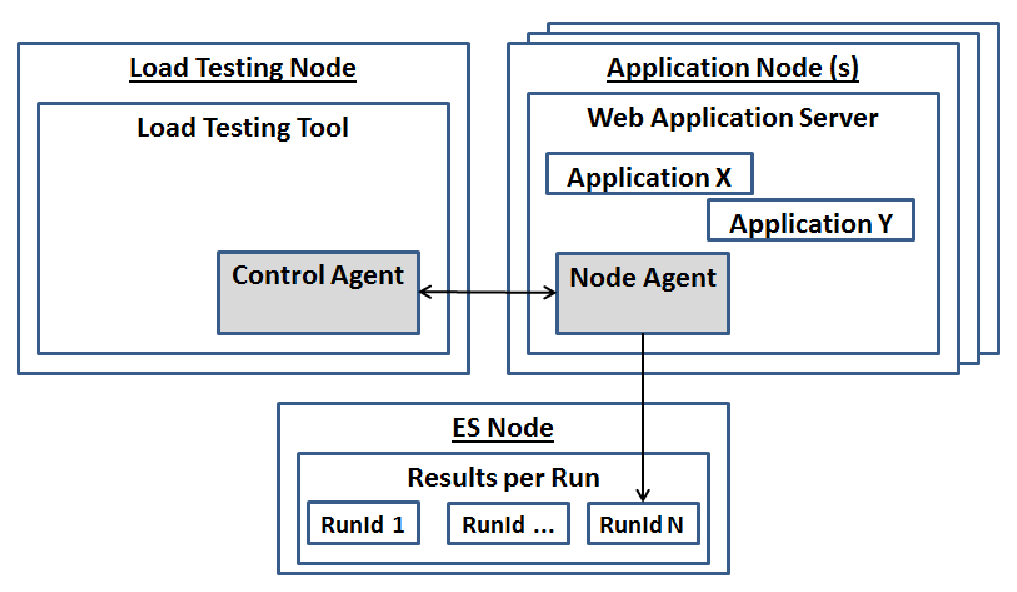
\includegraphics[totalheight=.3\textheight,width=0.9\textwidth]{architecture_dwait}
\caption{High-level Architecture of the solution}
\label{fig_Arch}
\end{figure}

It is important to highlight two assumptions that were considered when defining
the above design. As the scope of this work is the performance testing domain,
it is assumed that a Load Testing tool will always be present in the
testing environment. From the time been, the scope of this work is also focused
on Web Applications (a traditional Java business niche which is also type of 
applications that our industrial partner tests). For this reason, it is also
assumed at this stage that there will always be a Web Application Server in each
one of the application nodes. This assumption has the extra benefit that the
\emph{WAIT Node Agent} is a Web Application. As it uses plain HTTP protocol
to interact with the \emph{WAIT Control Agent}, a single version of \emph{WAIT
Node Agent} could interact with multiples types of \emph{WAIT Control Agent}
(as it is possibly necessary to have one per type of Load Testing Tool) or even
used independently.

Based on the concepts presented here, a prototype has been developed in
conjunction with our industrial partner IBM. The \emph{WAIT Control Agent} was
implemented as a Eclipse Plugin for the Rational Performance Tester (RPT)
\footnote{http://www-03.ibm.com/software/products/us/en/performance},
while the \emph{WAIT Control Agent} was implemented as a Java Web Application,
composed of a single servlet and a few utility classes. Internally, the
application reuses the data gathering scripts that are currently available for
WAIT \footnote{https://wait.ibm.com/\#page=dataCollectors}. In both cases,
one of the main reason to chose that technology (Eclipse Plugin and Web
Application) was that they are simple to install, as one of the main drivers of
this work is to reduce the testing effort.

Once installed, WAIT can now be configured as any other resource in RPT. This
scenario is shown in \figurename ~\ref{fig_config}. Similarly, once the performance
test has started, WAIT can now be monitored as any other resource in the
\emph{Performance Report} of RPT under the \emph{Resource View}. This is shown
in the \figurename ~\ref{fig_mon}. Finally, the WAIT report (which is initially created 
once the first upload is received and then updated after every data
upload) is also accessible within RPT, so that the tester does not need to
leave RPT during the whole duration of the performance test. This is shown
in \figurename ~\ref{fig_report}.

\begin{figure}[!h]
\centering
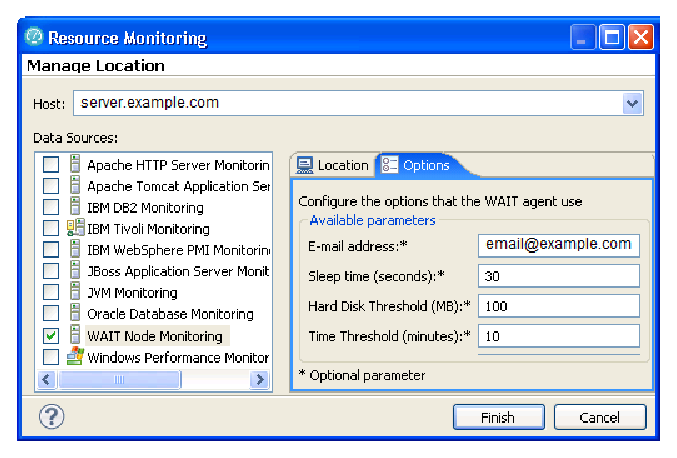
\includegraphics[totalheight=.3\textheight,width=0.8\textwidth]{WAIT-config}
\caption{WAIT configuration through RPT GUI}
\label{fig_config}
\end{figure}

\begin{figure}[!h]
\centering
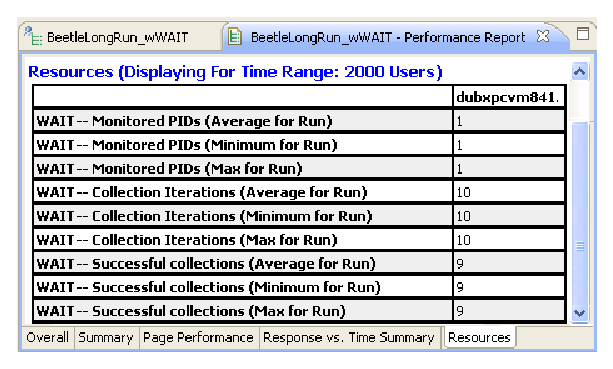
\includegraphics[totalheight=.3\textheight,width=0.8\textwidth]{WAIT-monitoring}
\caption{Monitoring of WAIT Node Agents through RPT}
\label{fig_mon}
\end{figure}

\begin{figure}[!h]
\centering
\includegraphics[totalheight=.4\textheight,width=1.0\textwidth]{WAIT-report}
\caption{WAIT Report available within RPT views}
\label{fig_report}
\end{figure}


%%%%%%%%%%%%%%%%%%%%%%%%%%%%%%%%%%%%%%%%%%%%%%%%%%%%%%%%%%%%%%%%%%%%%%%%%%%%%%%%%%%%%%%%%%%%%%%%%%%%%%%%%%%%
% Experimental Setup / Experiments
%%%%%%%%%%%%%%%%%%%%%%%%%%%%%%%%%%%%%%%%%%%%%%%%%%%%%%%%%%%%%%%%%%%%%%%%%%%%%%%%%%%%%%%%%%%%%%%%%%%%%%%%%%%%

\section{Experimental Evaluation}

In this section the experimental setup is presented along with the experiments themselves. 
After each experiment, its results are also discussed.

In total, 3 experiments were performed. The first two experiments pursed to
answer the research question 2 (How can the overhead be kept low during the whole 
performance test execution to avoid compromising the results?), while the third experiment
pursued to answer the research question 3 (What benefits in productivity can a tester 
achieve if the previous questions are answered?). Finally, the combined outcome
of the three experiments pursued to answer the research question 1 (How can the usage 
of WAIT be automated to minimize the effort required to use it in sync with the performance testing?).

During the evaluation phase 4 different types of nodes were required. An RPT
node, responsible of running the performance test, was a machine running Windows
XP with an Intel Xeon processor at 2.67 Ghz with 3GB of RAM using RPT 8.2.1.3.
A WAIT Server node, where the collected data was uploaded and the results
report was generated, was a machine running Red Hat Enterprise Linux Server 5.9,
with an Intel Xeon processor at 2.66 GHz with 2GB of RAM using Apache Web Server 2.2.3.
One or more application nodes, each one running a 64-bit Windows Server 2008,
with an Intel Xeon E7-8860 (4 cores) at 2.26 GHz with 4GB of RAM and Java 1.6.0
IBM J9 VM (build 2.6). Finally, a Load Balancing node (required in the presence
of multiple application nodes) had the same characteristics of the WAIT Server node using
mod\_jk with a round robin strategy for load balancing purposes.

The above nodes were arranged in 2 environment setups: For the first
experiment, a single application node configuration was used. This environment was composed of one RPT node, 
one application node and one WAIT Server node. For the second and
third experiments, the environment was composed of one RPT node, one load
balance node, two application nodes and one WAIT Server node. Furthermore all
machines are connected by a 10 GBit LAN.These environment set-ups are shown in \figurename ~\ref{fig_env}.

\begin{figure}[!h]
\centering
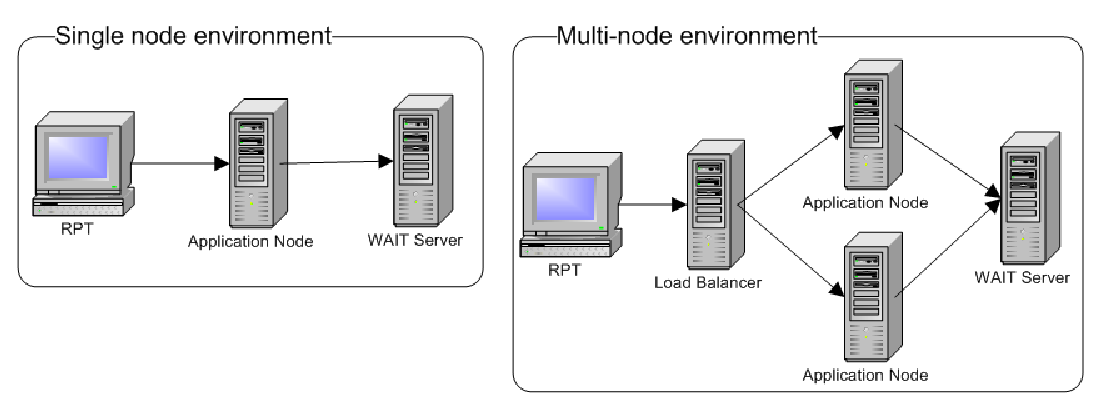
\includegraphics[totalheight=.25\textheight,width=0.8\textwidth]{Environments}
\caption{Environment Set-ups used in the Experiments}
\label{fig_env}
\end{figure}

\subsection{Experiment \#1}

Its objective was to validate that the proposed approach had a low overhead in
a single-node environment. This test involved the assessment of four metrics:
The throughput and response time (typical metrics used in performance testing) as well as CPU
and memory utilization (to assess how much additional resources the automation
requires). All metrics were collected through RPT (throughput and
directly, as RPT calculates them, while the resources' utilization was obtained
from the Windows Performance Monitor \footnote{http://technet.microsoft.com/en-us/library/cc768048.aspx} 
of each application node).

Two real-world applications were selected for this case study. The first
application was iBatis PetStore 4.0
\footnote{http://sourceforge.net/projects/ibatisjpetstore/} which is an 
upgraded version of the Sun's original J2EE Pet Store, popular e-commerce shopping 
cart application used to teach J2EE. This application was run over an Apache
Tomcat 6.0.35 Application Server \footnote{http://tomcat.apache.org/}. The
other application was IBM WebSphere Portal Server 8.0.1
\footnote{http://www-03.ibm.com/software/products/us/en/portalserver},
application which offers enterprise portal capabilities. This application was
run over an IBM WebSphere Application Server 8.0.0.5.
\footnote{http://www-01.ibm.com/software/webservers/appserv/was/}

For each applications, 3 WAIT combinations were tested: First the
application was executed without WAIT to get a baseline of how the
application performs by itself; then a manual WAIT execution (data collection
scripts directly executed with no upload) was introduced to measure how much
overhead WAIT adds by itself to the application; Finally, the automated approach was introduced to
measure how much overhead it adds. For each of the two combinations that have
WAIT present, two \emph{Sampling Interval} were considered: The first
value was 30 seconds and is the minimum suggested to avoid throughput slowdown
above 2\%). The second value was 480 seconds and was suggested by one expert in
our industrial partner.

All the other parameters involved in the setting up of the performance test were
suggested (as per their expert judgment) by our industrial partner as valid in a 
realistic test environment: A workload of 2,000 concurrent users; a duration of
1 hour; a \emph{Hard Disk Threshold} of 100MB; a \emph{Time Threshold} of 10
minutes. Finally, for each of the 10 identified combinations (5 per
application), 3 runs were performed. Each run was performed in an unloaded
single-node environment, where the corresponding Web Application Server was restarted 
before every run.

[[PENDING: 
\figurename XXXX shows the results of the experiments. 
Compare response time \& throughput with and without WAIT/WAIT-RPT.
Compare resource consumption per node with and without WAIT/WAIT-RPT.
Based on the above results we answer Q1 with Yes ...
Sanity checks: Not lost zip files, hard disk threshold respected?
To append results from excel file, they should include some tables
+ maybe a graphic of some type
+ Time in install/overall usage (easily estimated based in the high number of
test runs).
]]

\begin{table}[!h]
\caption{Selected GC Strategies}
\label{Selected_GCS}
\centering
\begin{tabular}{l|l|l}
\hline
\bfseries GC Strategy & \bfseries OldGen & \bfseries YoungGen\\
\hline
Serial & Mark Sweep Compact & Copy\\
Parallel & PS Mark Sweep & PS Scavenge\\
Concurrent & Concurrent Mark Sweep & Par New\\
\hline
\end{tabular}
\end{table}



\subsection{Experiment \#2}

Here the objective was to validate that the proposed approach keep experiencing
a low overhead even in a multi-node environment and in a longer run. This test
involved the same four metrics described in experiment \#1: Response time, throughput, CPU and memory utilization.

To compensate the increment in the duration of the tests, for this experiment 
only one application was selected: iBatis PetStore 4.0. Additionally, only 2 WAIT 
combinations were tested: First the application was executed alone to have a
baseline of how it performs by itself; then the automated WAIT approach was introduced 
to measure its overhead, using the \emph{Sampling Interval} of 480 seconds, as
suggested by the performance testing team of our industrial partner.

All the other parameters involved in the setting up of the performance test were
identical to the first experiment with two exemptions: The workload was
doubled to compensate for the additional application node and the
selected duration was 24 hours. Finally, each run was performed in an unloaded
multi-node environment, where all components were restarted before every
run.

[[PENDING: 
\figurename XXXX shows the results of the experiments.
Based on the above results we answer Q1 with Yes ...

Compare response time \& throughput with and without WAIT-RPT.
Compare resource consumption per node with and without WAIT-RPT.
Validate that there was not “information lost” between the collection and
uploading?

reliability! It might also help to show that the reliability of the solution
(I might take a look to other “fancy” NFR-related words)

To append results from excel file, they should include some tables
+ maybe a graphic of some type
+ Time in install/overall usage: Similarly to experiment 1 (easily estimated
based in the high number of test runs).
]]

\begin{table}[!h]
\caption{Selected GC Strategies}
\label{Selected_GCS}
\centering
\begin{tabular}{l|l|l}
\hline
\bfseries GC Strategy & \bfseries OldGen & \bfseries YoungGen\\
\hline
Serial & Mark Sweep Compact & Copy\\
Parallel & PS Mark Sweep & PS Scavenge\\
Concurrent & Concurrent Mark Sweep & Par New\\
\hline
\end{tabular}
\end{table}


\subsection{Experiment \#3}

The objective of this final experiment was to assess the benefits the approach
brings to a performance tester. For this experiment the automated approach to
use WAIT was used to monitor a modified version of iBatis PetStore 4.0 application 
which source code was modified to inject some performance issues to assess how 
WAIT was able to identify them and estimate the corresponding time savings.
Moreover, all other parameters involved in the setting up of the performance test 
were identical to the second experiment with exception of the test duration
which was 1-hour.


Specifically, 3 common performance issues were injected:
lockContentionBug -AAAA
heavyFileReadingBug -BBBB
databaseBug -CCCC

Figure 12 depicts aWAIT report on a 48-core system. TheWaiting Threads timeline shows a sudden and sustained surge of Blocked on Monitor; i.e. threads seeking a lock and not receiving it, and thus being blocked from making progress. Looking at the Cate- gory breakdown suggests that lock contention comes from miscel- laneous APACHE OPENJPA Code. The thread stacks from this cat- egory identify the location of the lock contention as line 364 of getMetaDataLocking(). Sometimes locking issues go beyond contention to the point of
deadlock or livelock. When WAIT detects a cycle in the monitor graph, their Wait State is Blocked on Deadlock. This situation ap- pears in Figure 13. Looking at the thread stacks at the lower right of the report suggests that the threads are waiting for a lock in the log- ging infrastructure method SystemOutStream.processEvent() line 277. Armed with this information, a programmer could look at the code and try to determine the reason for the deadlock.

Figure 16 presents an example of a database bottleneck. Unlike Fig- ure 11 where the database became completely unresponsive, in this case the database is simply struggling to keep up with the appli- cation server’s requests. Over time the server’s utilization varies between approximately 10% and 85%, and these dips in utilization correlate roughly with the spikes in the number of threads inWait- ing state Delayed by Remote Request and Category Getting Data from Database, thus pointing to the likely source of the delay. Clicking on the orange bar for Getting Data from Database
reveals the thread stacks that a developer can analyze to determine key parts of the application delayed by the database, and try to reduce the load generated against the database. Alternatively, the database could be optimized or deployed on faster hardware.

Figure 17 shows aWAIT report where filesystem activity is limiting performance. The top two pie charts and timelines show that there is enough Java code activity to keep the CPUs well-utilized. How- ever, the Waiting activity show a significant number of threads in Wait State Delayed by Disk I/O, and CategoryFilesystem Metadata Operations, suggesting room for improvement with faster disks, or by restructuring the code to perform fewer disk operations. Reducing these delays would clearly improve latency, since
each transaction would spend less time waiting on Disk I/O, but such improvement
would have other benefits as well. Even though the four CPUs on this machine are currently well utilized, this application will likely scale poorly on larger machines. As the number of processors increases, the frequent disk access delays will eventually become a scaling bottleneck. WAIT can help identify these scaling limiters early in the development process.


[[
PENDING:

- Results: Example of detected bugs!, simple and easy. All three bugs were
detected indicating their nature plus pinpointing which classes/methods within
the code were responsible.

lockContentionBug
heavyFileReadingBug
databaseBug
+ screen shoots!
Reduction Time: Early detection or trends (stress early detection).
Time: Early detection (avoid wasting resources if serious issues identified).
Average time of fixing an issue hard to know but even with a conservative
estimate . . . not bad.

Cost to locate defect = Cost of testing / the number of defects located
Increasing the TESTER PRODUCTIVITY

+ Logically estimated the benefits: Single report.
- Previously you would have ended with:
- X reports, assuming you monitored X nodes and generated all the reports after
the test execution finished.
- X*Y reports, assuming you monitored X nodes and generated the reports every
1/Y time.
- Now, in both cases you would have ended with a single report.

X,Y to an actual number (use case) … more qualitative, but showing how it is best 1 than many!

To conserve space, only the relevant portions of the UI
for each performance issue are presented.

The measures of success were the ability to identify performance problems that
affect the applications. Moreover, the tool should allow a wider range of
testers to perform the expert analysis, offering at the same time significant time savings for the expert users.

The results from using the tool were very encouraging the bugs were identified
as well as the time saved was quite high. The time saved per application is
around 1.6 hours: Split the time savings per type!

Another important detected advantage was the ability to open precise bugs.
Testers used the contextual information from the tool to investigate deeper the
issues and provide detailed description in the bug that they would open.
Furthermore, less experienced testers could also use this information to gain a
deeper understanding of these type of problems.

Two iterations were run: The first was done to catch up as many issues as
possible. The 2nd one shows the results report after fixing issues (possible an
intermediate run might be needed, as some issues might mask other ones) After each run, the detected bugs will be “fixed”.

In conclusion, the test case showed that the use of the automated approach
could have several advantages: The time saving from its usage is high.

Benefits: Less Time (setup, monitor, analysis, go/no-go decision) -> Less
Learning curve / Less Error-Prone, Share knowledge / experience (remain), “Real-time”, Keep as light-weight as possible (minimum add-ons + low overhead)
Time-consuming/complex data gathering (one data source per monitored process).
Time-consuming/Complex report analysis (one report per monitored process).
Plus required synchronization with the performance testing execution.
SME expertise required to interpret the reports: Problem with consumability in
parts of Dev, SVT, Perf and Support (few engineers outside of Watson are thread dump experts)
Important to rephrase it as estimated tester time benefit? (at least a high
level estimate … do not forget the time dimension!)
]]

\subsection{Threads to Validity}

Like any empirical work, there are a number of threats to the validity of these
experiments. The first one is the potential environmental noise could affect in
the testing environments considering that the environments are not isolated. To
mitigate the potential effect the noise might have in the obtained results, multiple runs 
were executed for each identified combination. Additionally, in order to know if
the differences between the obtained results were statistically significant (specially in cases 
were the differences were minimal, for example between the runs of the
applications alone against those runs using WAIT with a very low sample rate), the statistic Paired t-Test
\footnote{http://www.aspfree.com/c/a/braindump/comparing-data-sets-using-statistical-analysis-in-excel/}
was performed to determine if the null hypothesis (the changes in the
environment, practically the addition of WAIT in different forms, have no
impact in the environment) was rejected or not with 95\% of certainty.

Another thread is the selection of the performance testing parameters (i.e.
workload and duration of the test). This was addressed with the expert judgement 
of the SVT, which couched on the selection of those parameters that are
commonly used in the industry. Finally, the validity of these results are
threatened by the selection of the tested applications. Despite the fact that
they are real world applications and different in terms of functionality, their
limited number implies that not all types of applications have been tested and
one application with characteristics that are completely different might
generate different results. Wider experiments need to be executed to get more
general conclusions. However, in principle, there is no reason to believe that
the approach is not applicable to other environments.


%%%%%%%%%%%%%%%%%%%%%%%%%%%%%%%%%%%%%%%%%%%%%%%%%%%%%%%%%%%%%%%%%%%%%%%%%%%%%%%%%%%%%%%%%%%%%%%%%%%%%%%%%%%%
% Section 7: Conclusions
%%%%%%%%%%%%%%%%%%%%%%%%%%%%%%%%%%%%%%%%%%%%%%%%%%%%%%%%%%%%%%%%%%%%%%%%%%%%%%%%%%%%%%%%%%%%%%%%%%%%%%%%%%%%

\section{Conclusions and Future Work}

The identification of performance problems and the diagnosis of their root
causes are very complex and time-consuming activities in highly distributed
environments, which also tend to rely on the expertise of the involved
engineers. The objective of this work was to address the limitations that
prevent the usage of WAIT in the performance testing domain, so that WAIT can be
effective used to reduce the expertise and overall effort required to do
good performance analysis and to identify the root causes of those issues.
To achieve this goal the paper presented a novel automation approach and its
validation, composed of the implementation of a prototype and a study
case with two real-life applications. The results are encouraging as they have
proved that the approach addresses effectively the adoption barriers for WAIT in 
a distributed performance testing environment: The solution has proven being
light-weight, generating a low overhead ([PENDING]). Moreover, from a tester
usability perspective, there are also tangible time savings in terms of the
effort required to detect performance issues.

Future work will concentrate on assessing the practicability of the
approach and its benefits in a major scale through broader study cases with our
industrial partner IBM. It will also be evaluated how best to exploit the
additional functional information that can now be obtained from a tested environment
(i.e. test workload, response time, throughput and transactions) in order to
improve the qualitative and quantitative capabilities of the idle-time
analysis methodology (over which WAIT is based on) to identify more
types of performance problems.

%%%%%%%%%%%%%%%%%%%%%%%%%%%%%%%%%%%%%%%%%%%%%%%%%%%%%%%%%%%%%%%%%%%%%%%%%%%%%%%%%%%%%%%%%%%%%%%%%%%%%%%%%%%%
% Section 8: Acknowledgements
%%%%%%%%%%%%%%%%%%%%%%%%%%%%%%%%%%%%%%%%%%%%%%%%%%%%%%%%%%%%%%%%%%%%%%%%%%%%%%%%%%%%%%%%%%%%%%%%%%%%%%%%%%%%

\section*{Acknowledgments}

We would like to thanks Amarendra Darisa, from SVT IBM Dublin, as his expertise
and experience in performance testing helped us through the scope definition and validation of this work.

This work was supported, in part, by Science Foundation Ireland grant 10/CE/I1855 to Lero - the Irish Software Engineering Research Centre (www.lero.ie).

% Between 12 - 24 \ldots 18 sounds like a good number!
\bibliographystyle{splncs}
\bibliography{dwait_manual,dwait}

%\section*{Appendix: Springer-Author Discount}

\end{document}


• Links about common performance issues:
1. https://onyx.koli.ch/get/6448/3+-+Common+Web+Application+Errors.pdf
2. http://www.crn.com/slide-shows/cloud/231000374/10-most-common-causes-of-web-mobile-app-performance-issues.htm?pgno=1
3. www.tracelytics.com/blog/two-most-common-performance-mistakes/
4. http://gettingreal.37signals.com/toc.php
5. http://jonathanhui.com/top-j2ee-application-performance-problems



 ----------------------

 
 Related Work - First Draft / Ideas

Automated Performance Testing (support tools).
•	Performance Analysis Tools/Techniques (from WAIT papers).
•	WAIT

<<
(Intro) Related Techniques: In the software development process, performance testing is 
commonly conducted to determine an application's performance as experienced by the user.
In this context, the focus is generally not on a single application session but
on the application in its entirety, i.e., one does not test a single, isolated re-
quest of a single user but rather the performance when many users interact with
the application simultaneously. Software testers commonly use techniques such
as load testing, stress testing, etc., to perform these kinds of tests [3]. There
is a variety of commercial products and free open-source tools available for the
task. For example, IBM's Rational Performance Tester [4] and HPs LoadRunner
[5] both do scalability testing by generating a real work load on the application.
Open-source tools such as Apache's JMeter [6] and Grinder [7] provide a similar
functionality.
Motivated by the large cost for commercial performance testing tools, Chen
et al. created Yet Another Performance Testing Framework [8]. It enables users
to create custom test programs which dene the business operations to be per-
formed during the test. Chen's framework then executes these tasks concurrently.
In [9], Zhang et al. present a cloud-based approach to performance testing of web
services. Their system provides a frontend in which users can specify test cases
which are then dispatched to Amazon EC2 [10] cloud instances for execution.
Similar to all the previous tools, their system is testing the performance under
concurrent user access to the system.
[[
3. Molyneaux, I.: The Art of Application Performance Testing. Volume 1. O'Reilly
Media (2009)
4. IBM: Rational Performance Tester. http://www-01.ibm.com/software/
awdtools/tester/performance/
5. Hewlett Packard: HP LoadRunner. http://www8.hp.com/us/en/software/
software-product.html?compURI=tcm:245-935779
6. Apache Software Foundation: Apache JMeter. http://jmeter.apache.org/
7. Aston, P.: The Grinder, a Java Load Testing Framework. http://grinder.
sourceforge.net/
8. Chen, S., Moreland, D., Nepal, S., Zic, J.: Yet Another Performance Testing
Framework. In: Australian Conference on Software Engineering (ASWEC). (2008)
170 \{179
9. Zhang, L., Chen, Y., Tang, F., Ao, X.: Design and Implementation of Cloud-based
Performance Testing System for Web Services. In: Conference on Communications
and Networking in China (CHINACOM). (2011) 875 \{880
10. Amazon Web Services LLC: Amazon Elastic Compute Cloud (Amazon EC2).
http://aws.amazon.com/ec2/ (2012)
]]

Related Work: The idea of replaying a test execution in a simulator is, of course, not new. The
overall approach is frequently referred to as the capture and replay paradigm,
and has long been studied in different contexts such as testing of concurrent
programs [2]. ... To our best knowledge, our approach is the first to combine replay with model-based
methods for error detection within a test-case generator. Our contribution is not
a theoretical one, but comes from an industrial perspective.

Related Work: Unlike these approaches, our work aims at proposing a generic and platform
independent test system based on the TTCN-3 standard to execute runtime
tests. The proposed test system supports different test isolation mechanisms in
order to support testing different kinds of components: test sensitive, test aware
or even non testable components. Such test system has an important impact on
reducing the risk of interference between test behaviors and business behaviors
as well as avoiding overheads and burdens.

SPE, The commonest approach is purely measurement-based; it
applies testing, diagnosis and tuning late in the development cycle, 
when the system under development can be run and measured (see, e.g.
[2][4][8][9]).

[2] M. Arlitt, D. Krishnamurthy, J. Rolia, “Characterizing
the Scalability of a Large Web-based Shopping System'',
ACM Trans. on Internet Technology, v 1, 2001, pp. 44-69.

[4] A. Avritzer, J. Kondek, D. Liu, and E. J. Weyuker,
"Software performance testing based on workload
characterization," in Proc. WOSP’2002, Rome, , pp. 17-24.

[8] S. Barber, “Creating Effective Load Models for
Performance Testing with Incomplete Empirical Data”, in
Proc. 6th IEEE Int. Workshop on Web Site Evolution, 2004,
pp. 51-59.
[9] S. Barber, “Beyond performance testing”, parts 1-14,
IBM DeveloperWorks, Rational Technical Library, 2004,
www-128.ibm.com/developerworks/rational/library/4169.html

Performance testing on part or all of system, under
normal loads and stress loads [8]. The use of test data
to solve problems is the subject of [9]. This activity is
discussed in Section 3 below.

[8] S. Barber, “Creating Effective Load Models for
Performance Testing with Incomplete Empirical Data”, in
Proc. 6th IEEE Int. Workshop on Web Site Evolution, 2004,
pp. 51-59.
[9] S. Barber, “Beyond performance testing”, parts 1-14,
IBM DeveloperWorks, Rational Technical Library, 2004,
www-128.ibm.com/developerworks/rational/library/4169.html

Technical developments -> Visualization and diagnostics
Understanding the source of performance limitations is a search process, which
depends on patterns and relationships in performance data, often revealed by
visualizations. Promising areas for the future include better visualizations,
deep catalogues of performance-related patterns of behaviour and structure, and
algorithms for automated search and diagnosis.
Present visualization approaches use generic data exploration views such as
Kiviat graphs (e.g. in Paradyn [47]), traffic intensity patterns overlaid on
physical structure maps [47], CPU loading overlaid on scenarios, and breakdowns
of delay [66]. Innovative views are possible. For example, in [60] all kinds of
resources (not just the CPU) are monitored, with tools to group resources and
focus the view. The challenge for the future is to visualize the causal interaction of
behaviour and resources, rather than to focus on just one or the other.
[[
[47] Merson, P. and Hissam, S. “Predictability by construction” Posters of
OOPSLA 2005, pp 134-135, San Diego, ACM Press, Oct. 2005.
[60] J.A. Rolia, L. Cherkasova, R. Friedrich, “Performance Engineering for EA
Systems in Next Generation Data Centres”, Proc. 6th Int. Workshop on Software and Performance, Buenos Aires, Feb. 2007.
[66] C.U. Smith, L. G. Williams, Performance Solutions, Addison-Wesley, 2002
]]

Technical developments -> Bottleneck identification

a search for a saturated resource which limits the system, is a frequent
operation. In [21], Franks et al describe a search strategy over a model, guided by its structure and
results, and detects under-provisioned resource pools and over-long holding
times. It combines properties of resources and behaviour, for a “nested” use of
resources. It scales to high complexity, is capable of partial automation, and
could be adapted to interpret measured data. A multistep performance enhancement
study using these principles is described in [83].
Another search strategy purely over data ([9], part 7) focuses on reproducing
and simplifying the conditions in which the problem is observed. The actual diagnosis
of the cause (e.g. a memory leak) depends on designer expertise.
A bottleneck search strategy combining the data and the model could detect more
kinds of problems (e.g. both memory leaks and resource problems) and could
provide automated search assistance.
Patterns (or anti-patterns) related to bottlenecks have been described by Smith
and Williams [66] and others (e.g., excessive dynamic allocation, “one-lane bridge”).
For the future, more patterns and more kinds of patterns (on measurements, on
scenarios or traces) will be important. Patterns that combine design, model and
measurement will be more powerful than those based on a single source.
[[
[9] S. Barber, “Beyond performance testing”, parts 1-14, IBM DeveloperWorks,
Rational Technical Library, 2004, www-128.ibm.com/developerworks/rational/library/4169.html

[21] G. Franks, D.C. Petriu, M. Woodside, J. Xu, P. Tregunno, 
“Layered Bottlenecks and Their Mitigation”, Proc 3rd Int. Conf. on Quantitative
Evaluation of Systems, Riverside, CA, Sept. 2006.

[83] J. Xu, M. Woodside, and D.C. Petriu, 
“Performance Analysis of a Software Design using the UML Profile for
Schedulability, Performance and Time”, in Proc. 13th Int.
Conf. Modeling Techniques and Tools for Computer Performance Evaluation, Urbana,
USA, Sept. 2003 ]]

Scalability analysis and improvement is largely a matter of identifying
bottlenecks that emerge as scale is increased, and evolving the architecture. Future
scalability tools will employ advanced bottleneck analysis but will depend more
heavily on models, since they deal with potential systems.


•	Performance Testing Tools? (HP Load Runner, Jmeter, RPT).

[Pending to see where better to fit these points:]
Benefit: Tools usability, productivity increase (less time identifying issues and their root cause), any benefit in the consolidation (other than reducing from N*M reports to 1), i.e. trends in time and/or nodes (probably good input from performance team):
* How does the process currently work? (steps and time) i.e. ~2 hours debugging, 2-4 RCA + fixing OO
* Issues in different nodes sound like environmental ones?
* Issues in different times (kind of trending) might involve the application?
They refer to “end to end” testing … the most common issue are deadlocks.

He uses different tools:
- Heap dumps: WAIT?
- Thread dumps: WAIT (locks, contentions) … around every 5 - 10 mins / ISA (performance analysis kit based on Eclipse).
- Overall development expertise (i.e. architecture, layers, frameworks, tools).
- Code profiling: tprof to profile in real time (recording every 1-2 mins to know the CPU usage per transactions); jprofiling (single transaction costs, such as CPU usage).
- Database: Tunning of SQL queries (or expert systems that encapsulate the identification of the most common issues).
- GC: gclite (expert system) or jmap.

Today, the state of industrial performance measurement and testing techniques is
captured in a series of articles by Scott Barber [8][9] including the problems
of planning, execution, instrumentation and interpretation.

[8] S. Barber, “Creating Effective Load Models for Performance Testing with
Incomplete Empirical Data”, in Proc. 6th IEEE Int. Workshop on Web Site Evolution, 2004,
pp. 51-59.
[9] S. Barber, “Beyond performance testing”, parts 1-14, IBM DeveloperWorks,
Rational Technical Library, 2004, www-128.ibm.com/developerworks/rational/library/4169.html

The tools used by performance analysts range from load generators, for supplying
the workload to a system under test, to monitors, for gathering data as the
system executes.

Key message/conclusion: The identification of the root causes of performance issues, relies very heavy on the expert knowledge of the user + requires a lot of different tools. There is no possible to indicate an average time per issue identification, but overall is very challenging/time-consuming.

 
 ----------------------------
  
  PENDING:
  - Complete the related work section.
  - Finalize the Pair T-Test analysis.
  - Try to merge the results of the WAIT report and tell some history
  (Environmental issues possible in Stand-By if the real report does not work).
  - Re-read the paper to see if it makes sense (i.e. the verbiage of the
  reserch questions should change to make a better fit with the experiments
  and their results).
  